
\section[Leyes clásicas de Mendel]{Leyes clásicas de Mendel: Las bases de la genética}

Si bien la genética ya había dado sus primeros pasos con Charles Darwin y su teoría de la evolución, esta teoría solo explicaba que los organismos llevan a cabo procesos de adaptación a su entorno y, en base a estos, evolucionan, sin embargo, el mecanismo detrás de estas adaptaciones seguía sin ser conocido. 

Gregor Mendel, un monje austriaco influenciado por el trabajo de Darwin, fue quien llevó a cabo el experimento que resultó en la creación de las bases de la genética.

\marginpar{\begin{minipage}{\marginparwidth}
\begin{figure}[H]
    \centering
    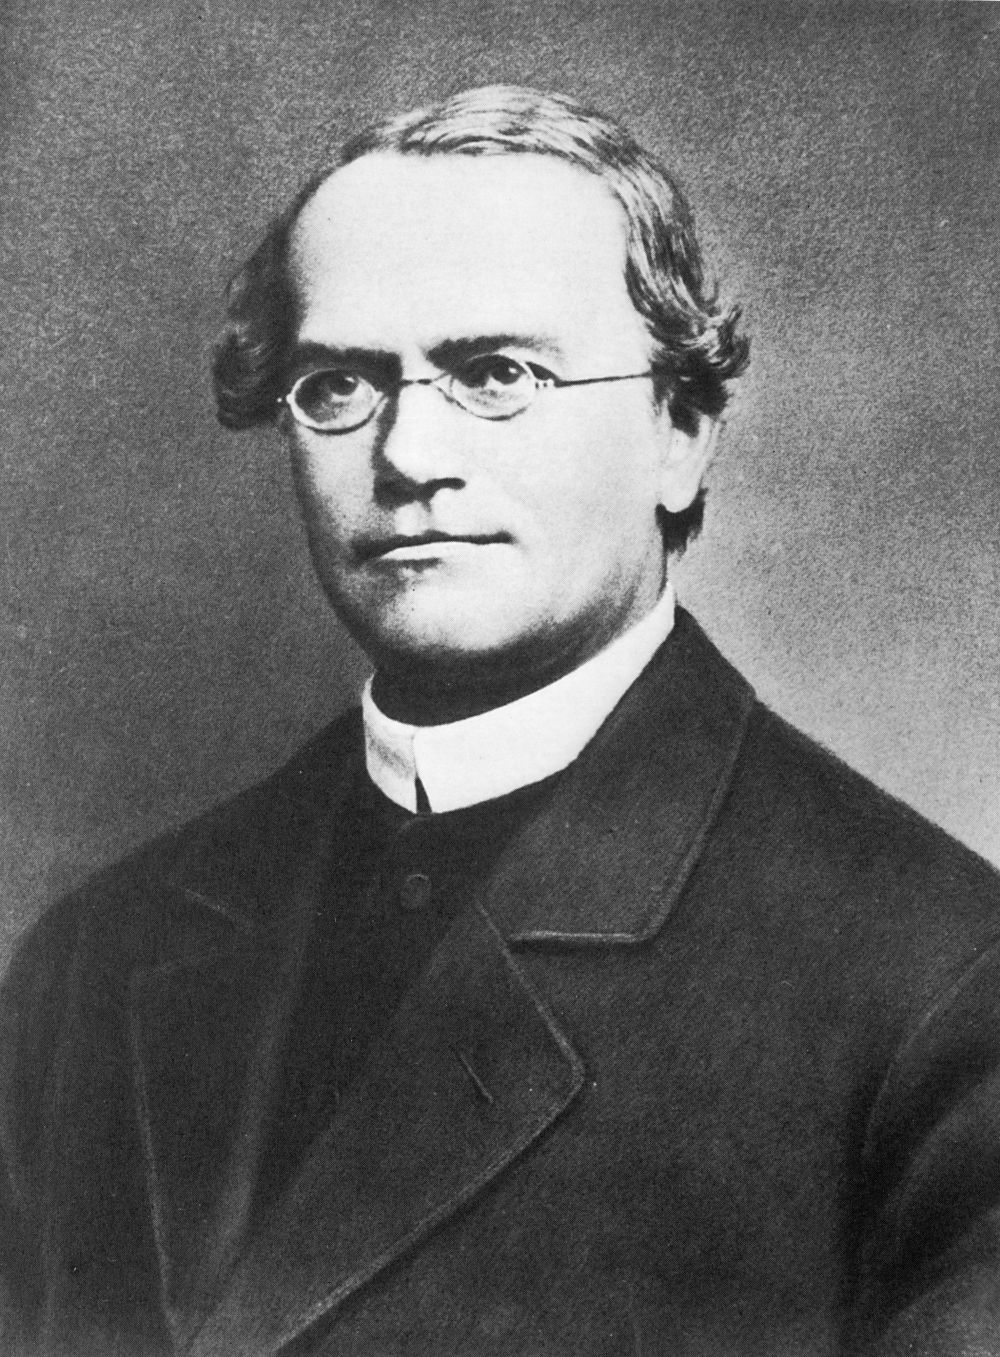
\includegraphics[width=\linewidth]{images/fig:gregor_mendel}
    \rule{\linewidth}{0.5pt}
    \caption[Retrato de Gregor Mendel]{Gregor Mendel, conocido como el padre de la genética}
    \label{fig:gregor_mendel_retrato}
\end{figure}
\end{minipage}}

Su experimento duró 7 años, de 1856 a 1863, y consistió en la reproducción controlada de la planta \sci{Pisum sativum}. Primero que nada Mendel se dedicó a generar lineas de guisantes ``puras'', o sea, que expresaban una característica definida, esto aprovechando la capacidad de autofecundación de \sci{P. sativum}. Una vez que tenía lineas puras, Mendel eliminó las anteras de las plantas (las estructuras que permiten tal autofecundación) para evitar que tal autofecundación interfiriera con las fecundaciones controladas que quería realizar. Asímismo, cubrió las flores para evitar que estas fueran fecundadas por factores como los insectos. Con estas prácticas como control, Mendel podía relacionar de manera confiable las características expresadas por la planta con los cruzamientos que realizaba entre las plantas. 

\marginpar{\begin{minipage}{\marginparwidth}
    \begin{figure}[H]
        \centering
        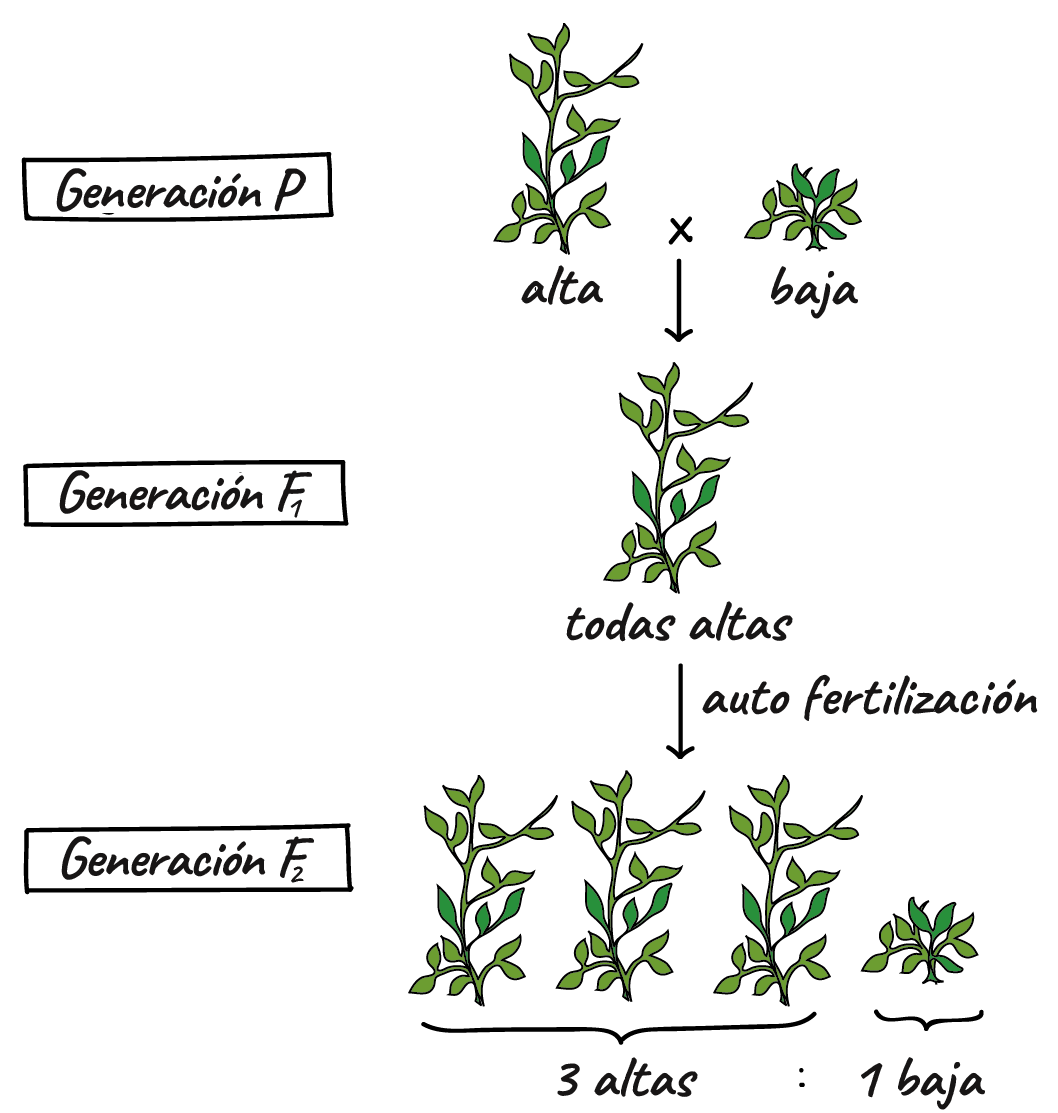
\includegraphics[width=\linewidth]{images/fig:experimentos_de_mendel}
        \rule{\linewidth}{0.5pt}
        \caption{Esquema de los experimentos de Gregor Mendel}
        \label{fig:experimentos_de_mendel}
    \end{figure}
\end{minipage}}

Lo primero que notó fue la dominancia de ciertos rasgos sobre otros. Partiendo de lineas puras (generación P), realizó cruces entre estas para obtener una generación ``hija'', o generación F\sub{1}\footnote{Generación filial, proviniendo filial de \textit{filius}, que significa ``hijo'' en latín}). Notó en estas nuevas plantas que ciertos rasgos dominaban sobre otros, por ejemplo, que al cruzar plantas altas y bajas, todas las plantas eran altas; o que al cruzar plantas con chícharos verdes y otras con chícharos amarillos, todas daban chícharos amarillos. Mendel llamó a los rasgos que si se mostraban \emph{rasgos dominantes}, mientras que llamó a las formas no expresadas \emph{rasgos recesivos}. 

Mendel dejó también que esta generación F\sub{1} se autofecundara, dando pie a la generacion F\sub{2}. En esta nueva generación encontró que el rasgo anteriormente no expresado, el rasgo recesivo, volvía a aparecer. Notó también que de cada 4 plantas altas en la generación F\sub{2}, 1 de ellas volvía a ser baja, o sea, que esta ``reaparición'' seguía una proporción 3:1.

Mendel explicó esto y el fenómeno anterior al establecer que existían \emph{factores hereditarios}, lo que hoy día llamamos \emph{genes}. Para explicar los fenómenos antes vistos en sus experimentos teorizó que cada individuo debía tener 2 copias de cada gen. A este par de copias hoy día se le denomina \emph{alelos}, y si tales \emph{alelos son iguales} se considera que el individuo es \emph{homocigoto} respecto a tal característica, mientras que si los \emph{alelos son diferentes} entre sí, entonces se denomina que el individuo es \emph{heterocigoto} para tal característica.

\begin{figure}[H]
    \centering
    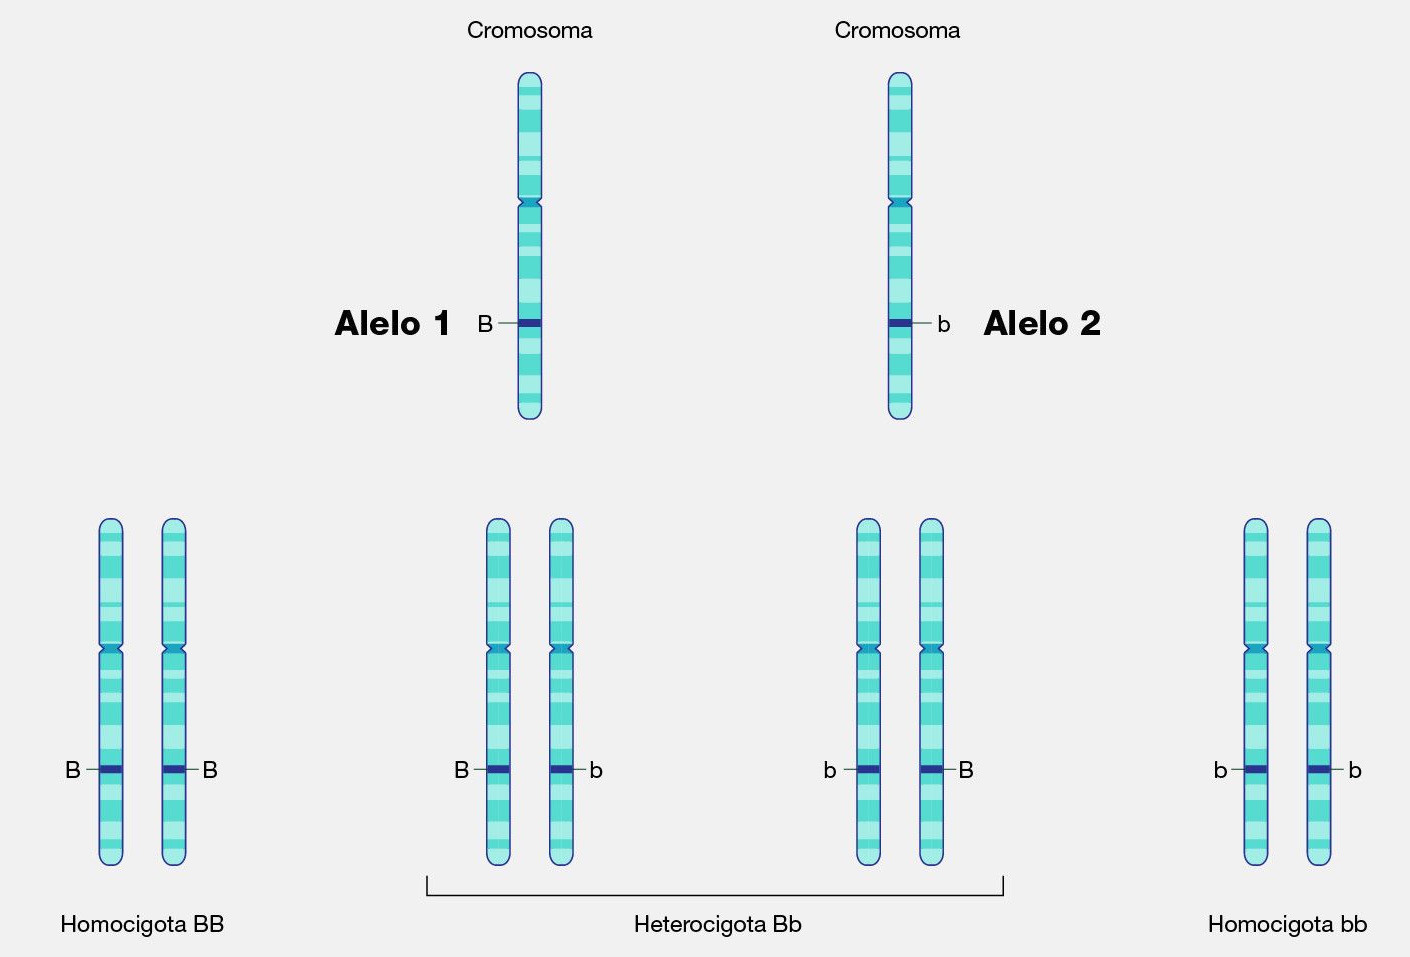
\includegraphics[width=\linewidth]{images/fig:alelos_homocigotos_heterocigotos}
    \rule{\linewidth}{0.5pt}
    \caption[Alelos homo y heterocigotos]{Las copias de un mismo gen se denominan alelos. Estos pueden ser homocigotos si son iguales o heterocigotos si son diferentes.}
    \label{alelos_homocigotos_heterocigotos}
\end{figure}

Mendel estableció que, al reproducirse, cada progenitor debía aportar 1 de sus alelos, y que si el individuo resultante era heterocigoto, uno de los alelos podría ocultar al otro, explicando los rasgos dominantes y recesivos. Asímismo, esta visión explica también la relación 3:1 que vió en la generación F\sub{2}.

\marginpar{\begin{minipage}{\marginparwidth}
    \begin{figure}[H]
            \centering
            \resizebox{\linewidth}{!}{\definecolor{Dominante}{RGB}{255,236,155}
\definecolor{Recesivo}{RGB}{187,210,142}
\begin{tikzpicture}[
    etiqueta/.style={font=\sffamily},
    individuo/.style={draw, circle, align=center, text width=0.75cm, font=\sffamily},
    alelo/.style={draw, diamond, font=\sffamily\scriptsize},
    tabla/.style={anchor=west, font=\sffamily\scriptsize},
    linea/.style={-Stealth, line width=0.5pt}
]

\node[etiqueta] (generacion p)  at (0,0)  {Generación P};
\node[etiqueta] (generacion f1) at (0,-2) {Generacion F\sub{1}};
\node[etiqueta] (generacion f2) at (0,-6) {Generacion F\sub{2}};
\node[individuo, fill=Dominante] (progenitor1) at ([xshift=2.5cm]generacion p) {AA};
\node[individuo, fill=Dominante] (progenitor2) at ([xshift=3cm]progenitor1) {aa};
\node[individuo, fill=Dominante] (hijo) at ([xshift=4cm]generacion f1) {Aa};
\node[alelo, fill=Dominante] (alelo1) at ([xshift=-1cm,yshift=-2cm]hijo) {A};
\node[alelo, fill=Recesivo] (alelo2) at ([xshift=1cm, yshift=-2cm]hijo) {a};

\node[tabla] (tabla combinaciones) at ([xshift=0.5cm]generacion f2.east) {
    \begin{tabular}{c|c}
        \colorbox{Dominante}{AA} & \colorbox{Dominante}{Aa} \\ \hline
        \colorbox{Dominante}{Aa} & \colorbox{Recesivo}{aa} \\ 
    \end{tabular}
};

\node[tabla] (tabla probabilidades) at ([xshift=0.5cm]tabla combinaciones.east) {
    \begin{tabular}{c|c}
        \colorbox{Dominante}{25\%} & \colorbox{Dominante}{25\%} \\ \hline
        \colorbox{Dominante}{25\%} & \colorbox{Recesivo}{25\%} \\
    \end{tabular}
};

\draw[linea] (progenitor1.south) to[out=-90,in=135] (hijo.north west);
\draw[linea] (progenitor2.south) to[out=-90,in=45]  (hijo.north east);
\draw[linea] (hijo.south) to[out=-90,in=90] (alelo1.north);
\draw[linea] (hijo.south) to[out=-90,in=90] (alelo2.north);
\draw[linea] (alelo1) to[out=0,in=90] ([xshift=0.25cm,yshift=0.5cm]tabla combinaciones.north east);
\draw[linea] (alelo2) to[out=180,in=90] ([xshift=0.25cm,yshift=0.5cm]tabla combinaciones.north east);
\draw[linea] (tabla combinaciones.east) -- (tabla probabilidades.west);
\end{tikzpicture}}
            \rule{\linewidth}{0.5pt}
            \caption[Simplificación del flujo de alelos en los experimentos de Mendel]{Diagrama mostrando de manera simplificada el flujo de alelos en el los experimentos de Mendel. La tabla final muestra el origen de la relación 3:1 que este observó.}
            \label{fig:diagrama_de_punett}
        \end{figure}
\end{minipage}}

A partir de este experimento podemos identificar también los conceptos de \emph{genotipo} y \emph{fenotipo}. Mientras que el genotipo consiste en todos los genes de un individuo, el fenotipo a las características físicas que expresa un individuo a partir de su genotipo.\citep{delcastilloruizGeneticaClinica2019} Por ejemplo, los chícharos de la generación F\sub{1} contaban con los genes tanto del color amarillo como del verde, ambos genes conforman parte de su genotipo; por otro lado, el fenotipo consiste en la característica expresada, en este caso, el color amarillo.

Todos estos conocimientos generados a partir de los experimentos de Mendel se han resumido en las \emph{Leyes de Mendel}:

\begin{enumerate}
    \item Al cruzar dos razas puras (homocigóticas) para un mismo carácter, todos los descendientes de la primera generación filial (F\sub{1}) son iguales entre sí (tanto en fenotipo como en genotipo) y presentan el carácter dominante de uno de los progenitores.
    \item Los dos alelos que determinan un carácter se separan o segregan durante la formación de los gametos (células sexuales). Cada gameto recibe solo uno de esos alelos.
    \item Los alelos de genes diferentes se transmiten a la siguiente generación de manera independiente unos de otros
\end{enumerate}

\marginpar{ {\rule{\marginparwidth}{1pt}} \footnotesize
    Las Leyes de Mendel y sus principios aplican unicamente a organismos que se reproducen sexualmente.
}


A pesar de los grandes hallazgos realizados por Mendel, cuando estos fueron publicados en 1866 no recibieron ninguna atención por parte de la comunidad científica. Los intentos de Mendel de recrear sus experimentos con otras especies de plantas del género \sci{Hieracium} fracasaron porque, como se descubriría hasta 1903, estas plantas tienen mecanismos particulares de reproducción. Gregor Mendel falleció en 1884 mientras la comunidad científica desconocía la existencia de sus ideas.

Alrededor del año 1900 varios investigadores terminaron por llegar a las mismas conclusiones que Mendel, y algunos de ellos redescubrieron su trabajo. Uno de ellos, William Bateson, no solo fue el primero en dar noticia de los trabajos de Mendel a la comunidad científica, sino que se convirtió en un gran defensor de sus hallazgos, lo que le valió el apodo de ``el bulldog de Mendel''. Además de esto, introdujo varios términos básicos como ``genética'' y ``alelo''. Estos aportes de Biteson, así como el descubrimiento de estructuras como los ácidos nucléicos y los cromosomas, hizo posible que la genética emergiera como una nueva ciencia.